\documentclass{beamer}
% % Example from http://www.math.umbc.edu/~rouben/beamer/quickstart-Z-H-3.html#node_sec_3
%\usepackage{default}
\usetheme{default}
\usepackage[utf8]{inputenc}  % this allows latex to understand UTF
                             % encoding in the file. This is
                             % important for Icelandic characters.
\usepackage[T1]{fontenc} % this enables icelandic characters in the output

\usepackage[caption=false]{subfig}

% % Use the UMBC theme
% Template derived from hfc.tex by
% Rouben Rostamian <rostamian@umbc.edu>
% August 31, 2004 
\usetheme{ru1}
\useinnertheme{ruboxes}
\setbeamercolor{ruboxes}{bg=violet!12,fg=black}

\usepackage{rotating} % for defining \schwa
\newcommand{\schwa}{\raisebox{1ex}{\begin{turn}{180}e\end{turn}}}

\title{GeoLog}
\subtitle{Milestone presentation}
\author[P. Helgasson, S. Ólafsson, S. Magnússon, \& Þ. Tómasarson]{Páll Helgason pallsh12@ru.is, Sindri Ólafsson sindrio12@ru.is, Sveinn Elmar Magnússon sveinnm12@ru.is, \& Þór Tómasarson thortom12@ru.is}
\institute[RU]{
  Department of Science and Engineering (TVD) \\
  Reykjavík University \\
}
\date{October 28, 2014} %% Put the real presentation day so it doesn't
                        %% change later
\begin{document}

%----------- titlepage ----------------------------------------------%
\begin{frame}[plain]
  \titlepage
\end{frame}

%----------- slides ----------------------------------------------%
\begin{frame}{Introduction}
	\begin{itemize}
	% sett each as seperate slide...
	\item Geological data collector
	\item Collects data from multiple sensors and sends the data over the world wide web. 
	\item Eases the observation of wide terrain
	\end{itemize}
	\begin{figure}
			\centering
	        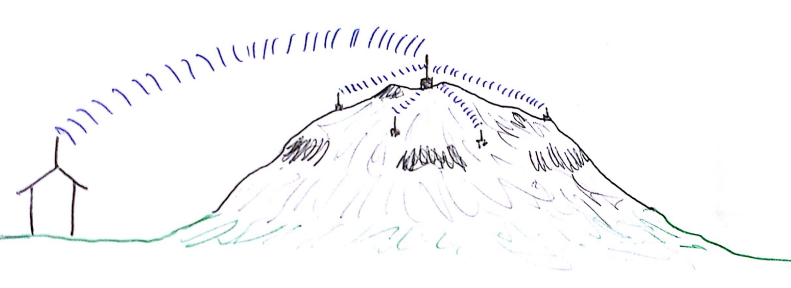
\includegraphics[height=3cm]{graphics/GeoLog.PNG}
	        \caption{Datalogging\cite{Helgason2014}}
	\end{figure}
\end{frame}

\begin{frame}{Introduction}
\begin{itemize}
\item Andrew D. Wickert cares.
\end{itemize}
\centering
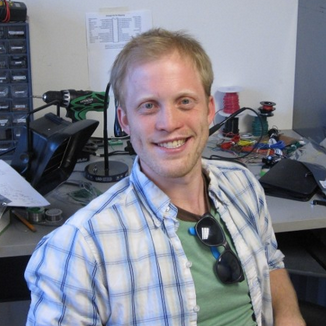
\includegraphics[height=5cm]{graphics/andrewWickert.png}
\cite{andrewWickert}
\end{frame}

\begin{frame}{Similar products}
\begin{figure}
  \centering
  \subfloat[\$3500\label{fig:a}\cite{WeatherShop2014}]
  {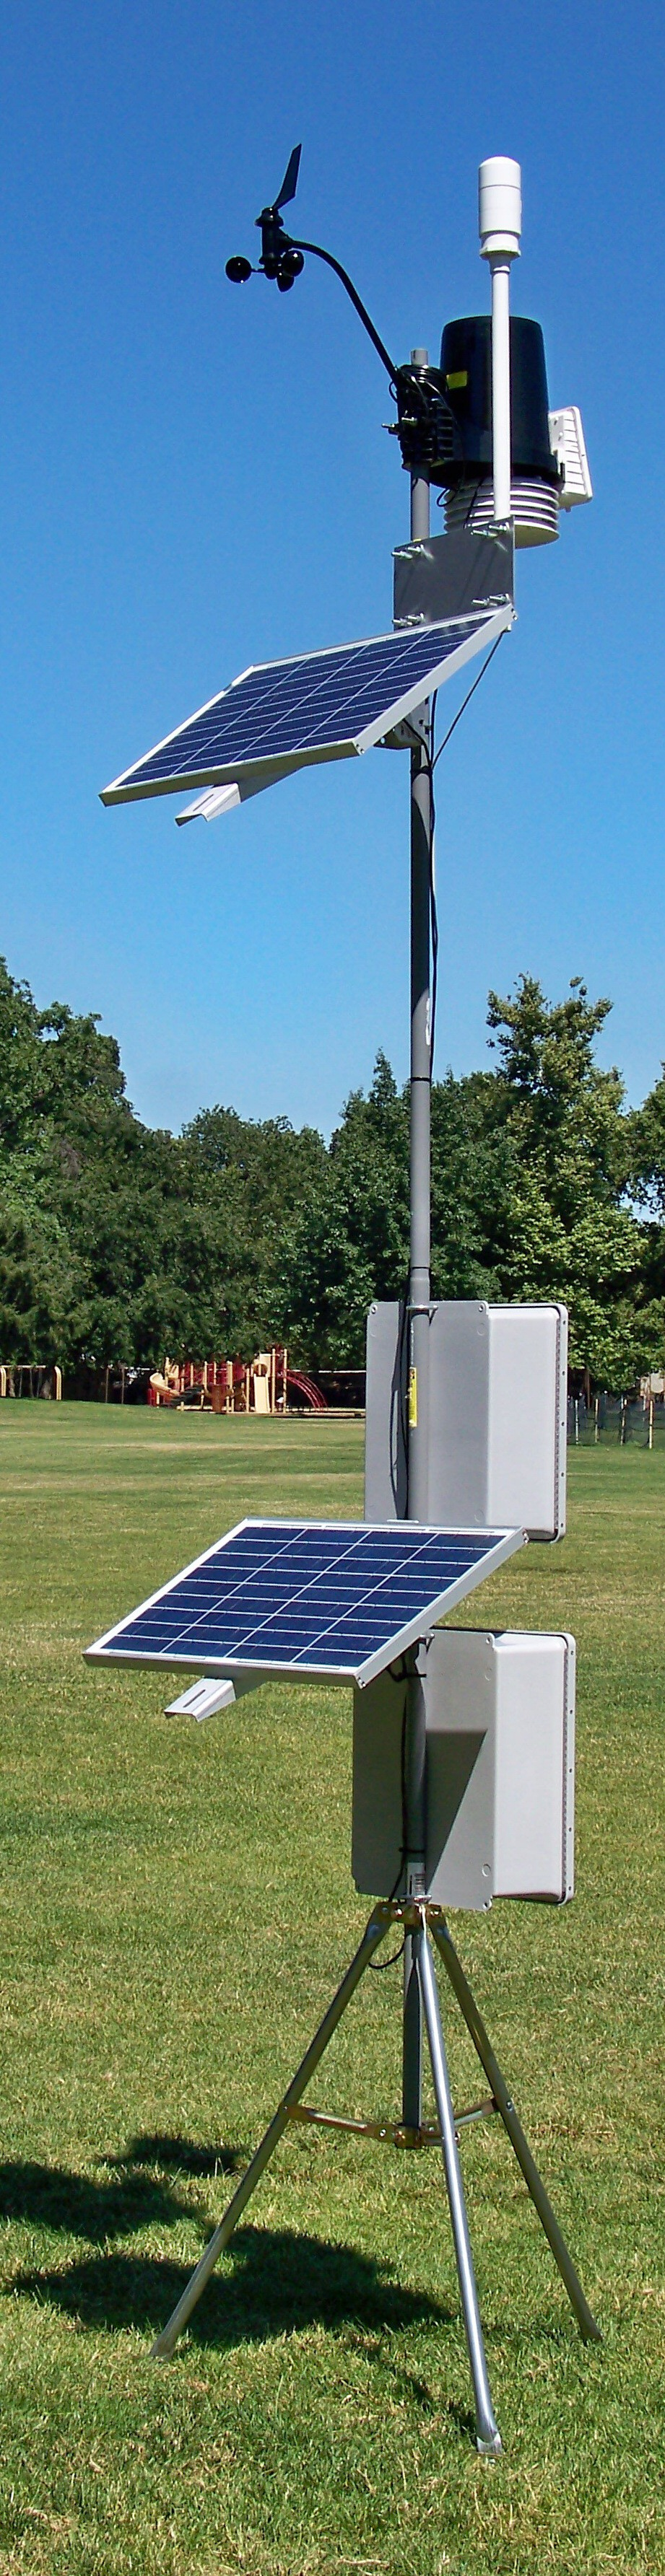
\includegraphics[height=5cm]{graphics/cellular_weather_station.JPG}}\quad
  \subfloat[\$2800\label{fig:b}\cite{TexasWeatherInstruments2014}]
  {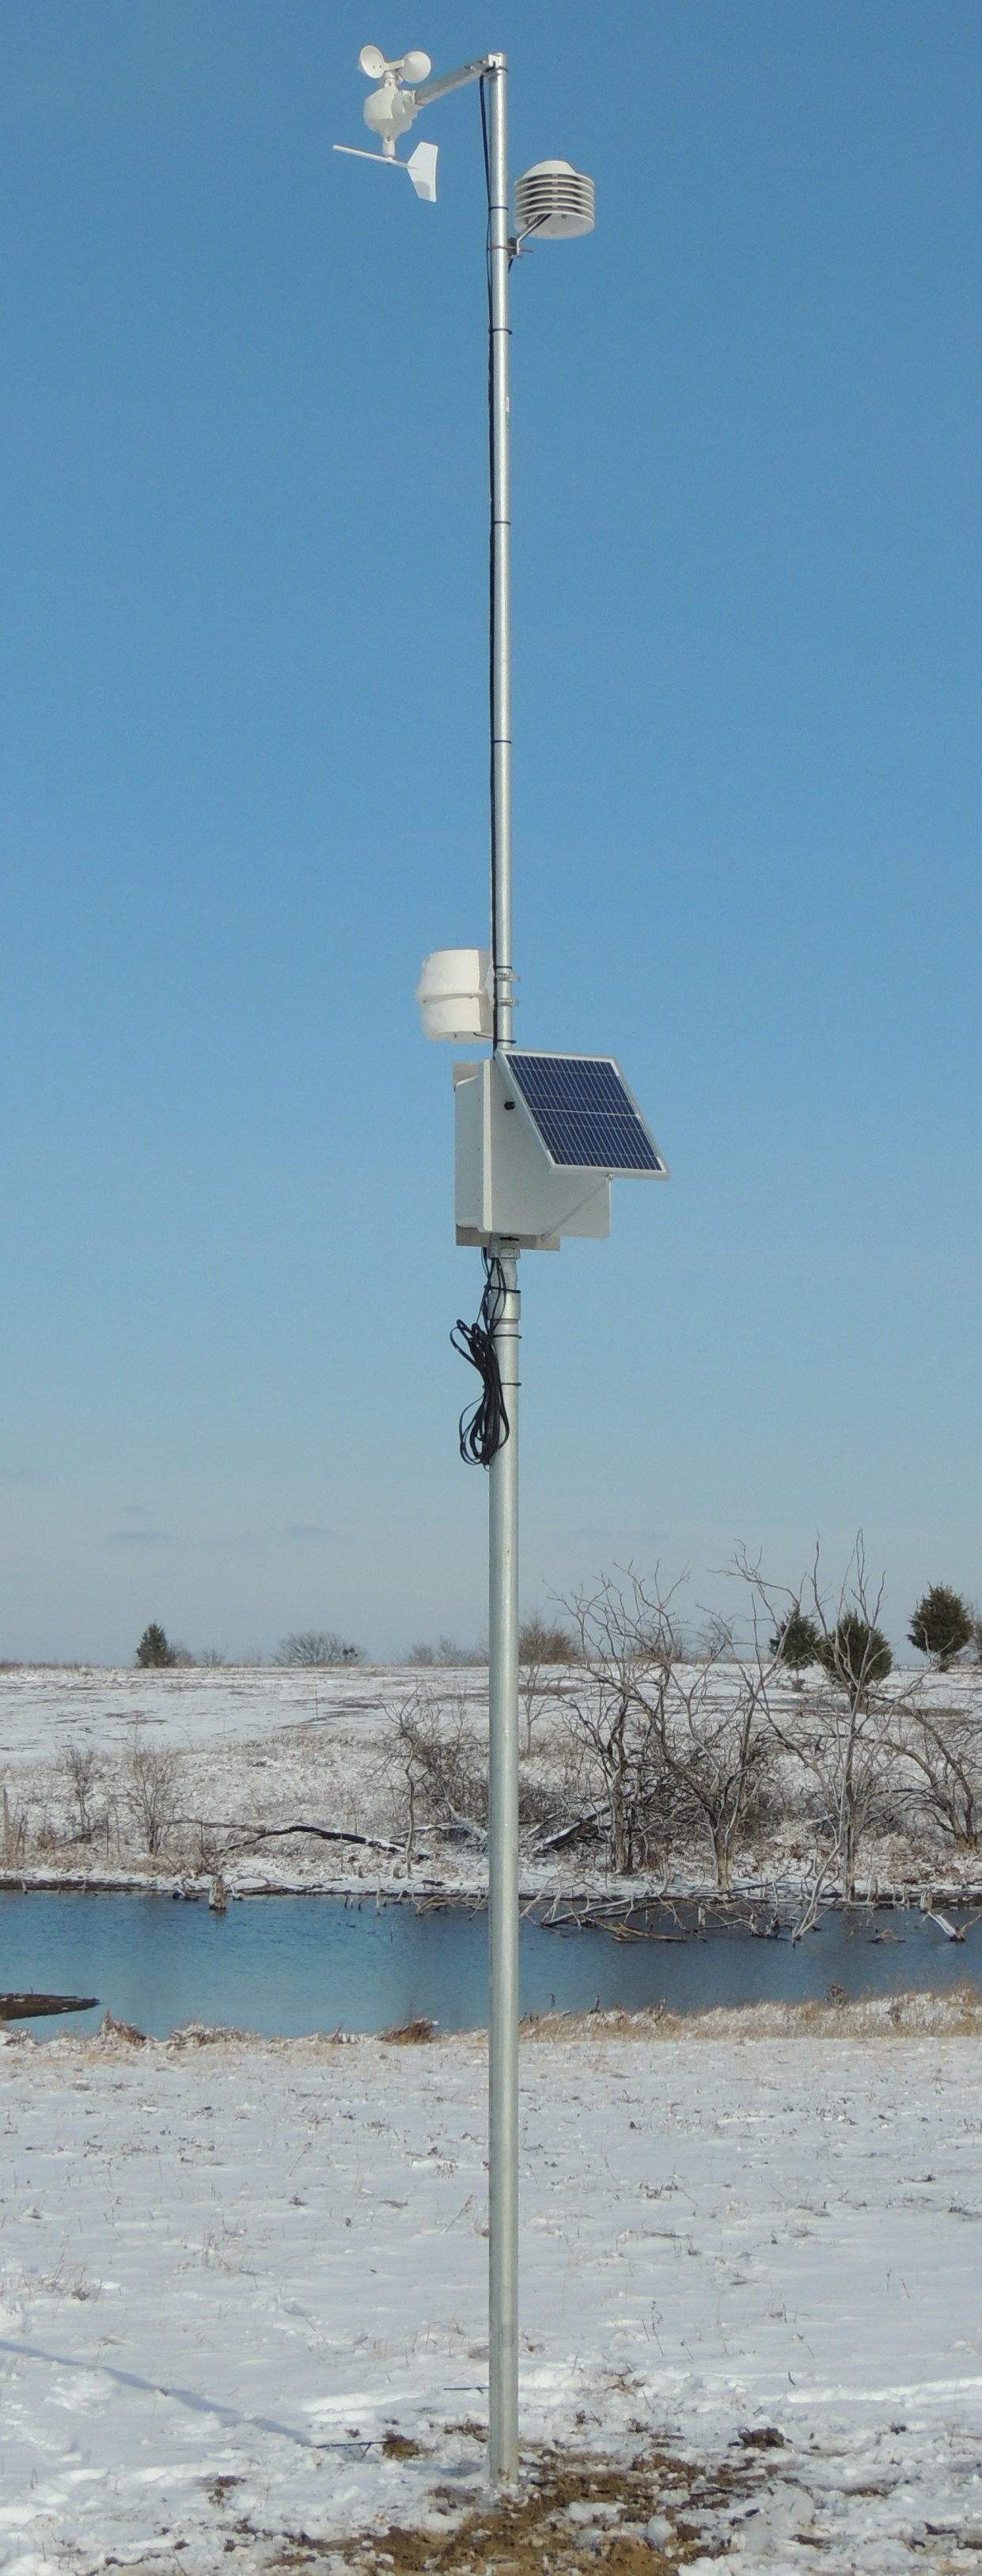
\includegraphics[height=5cm]{graphics/RWS-Snow.JPG}}\quad
  \subfloat[\$658\label{fig:c}\cite{Scientific2014}]
  {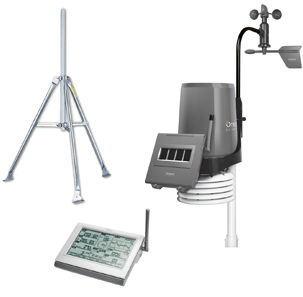
\includegraphics[height=3cm]{graphics/Oregon_Scientific_Pro_weather_system.PNG}}\quad
  \subfloat[\$595\label{fig:d}\cite{Davis2014}]
  {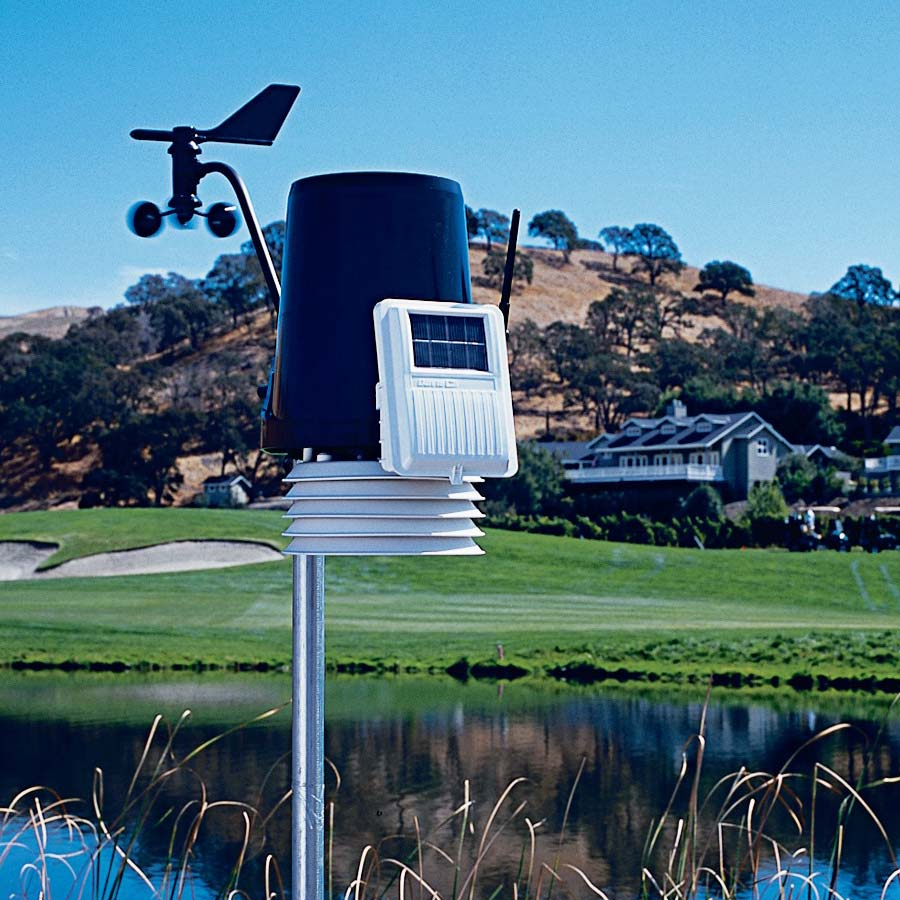
\includegraphics[height=3cm]{graphics/Davis_Vantage_Pro_2.JPG}}  
  \caption{Various price of weather stations}
  \label{fig:1}
\end{figure}
\end{frame}

\begin{frame}{Use case}
	\begin{itemize}
	\item Deployment of sensors
	\item Connect the sensors to communicators
		\begin{itemize}
		\item Wixel
		\item Xbee
		\item Any other wireless communicator
		\end{itemize}
	\item Position the main GeoLog module
	\item Connect to the Internet to see the incoming data
	\end{itemize}
	\begin{figure}
			\centering
	        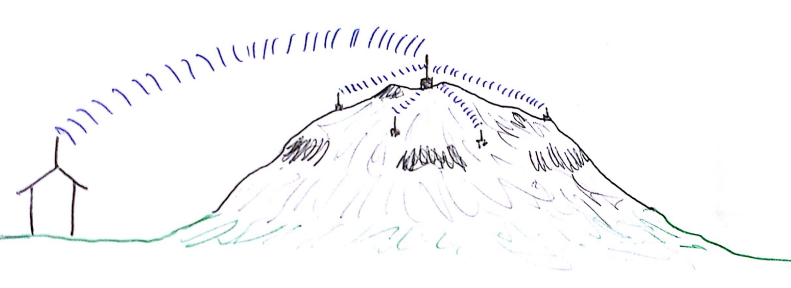
\includegraphics[height=3cm]{graphics/GeoLog.PNG}
	        \caption{Datalogging\cite{Helgason2014}}
	\end{figure}

\end{frame}

\begin{frame}{Design: Layering}
\centering
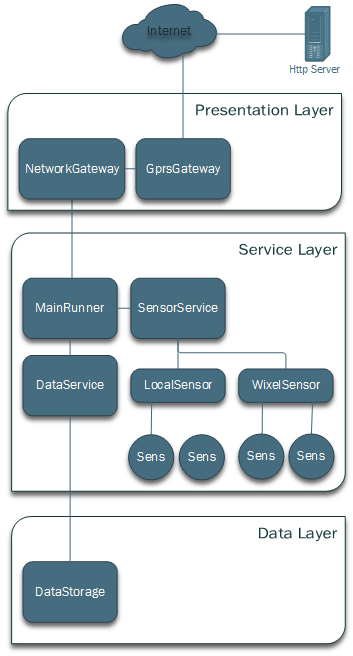
\includegraphics[height=7cm]{graphics/Layering.png}
%What are the pieces of your design (software, hardware, etc.)  and how
%do they work together?  Put some pictures here to help explain what is
%going on.  Remember to cite all pictures and text using BibTeX.  If you cited
%the textbook\cite{carryer2011IntroMechatronics}, that is what it would
%look like.
\end{frame}

\begin{frame}{Design: Software}
\centering
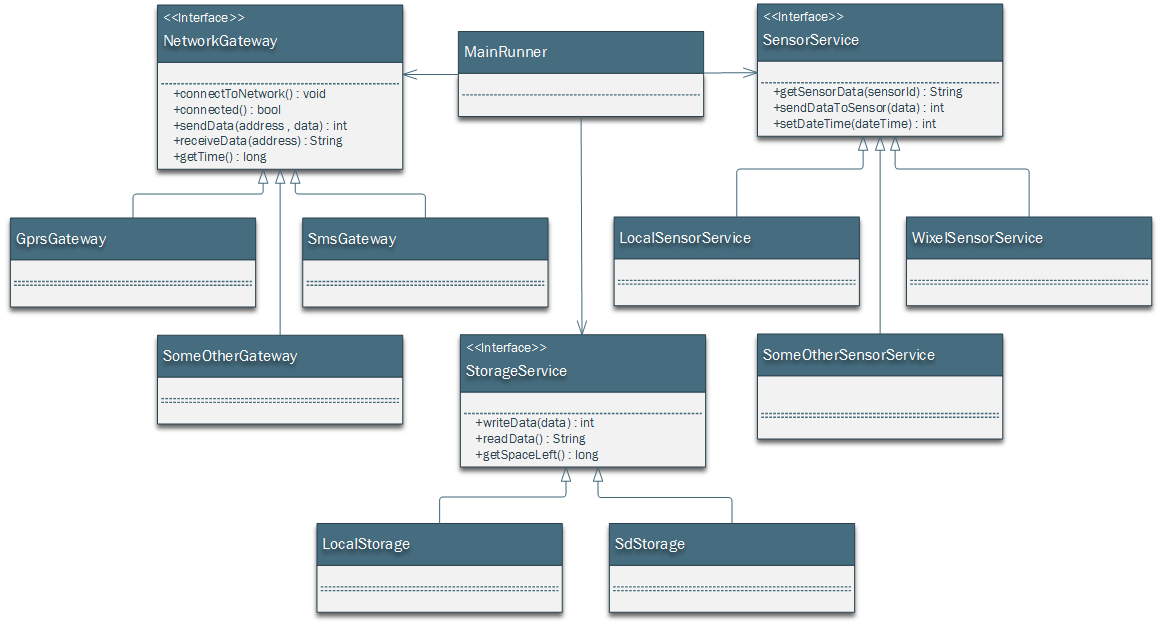
\includegraphics[width=11.5cm]{graphics/ClassDiagram.png}
\end{frame}

\begin{frame}{Design: Bill of materials (BOM)}

\begin{itemize}
\item 1 x Arduino Mega (Model: 2560 R3 from Sparkfun) \$45.95
\item 1 x GSM Module with shield  (Model: SM5100B from Sparkfun) \$99.95
\item 3 x Wixel   (With CC2511F32 microc. from Sparkfun) \$19.95
\item 3 x Sensors
\end{itemize}
\end{frame}

\begin{frame}{Status}
\begin{itemize}
\item GSM Arduino communication
\end{itemize}
\centering
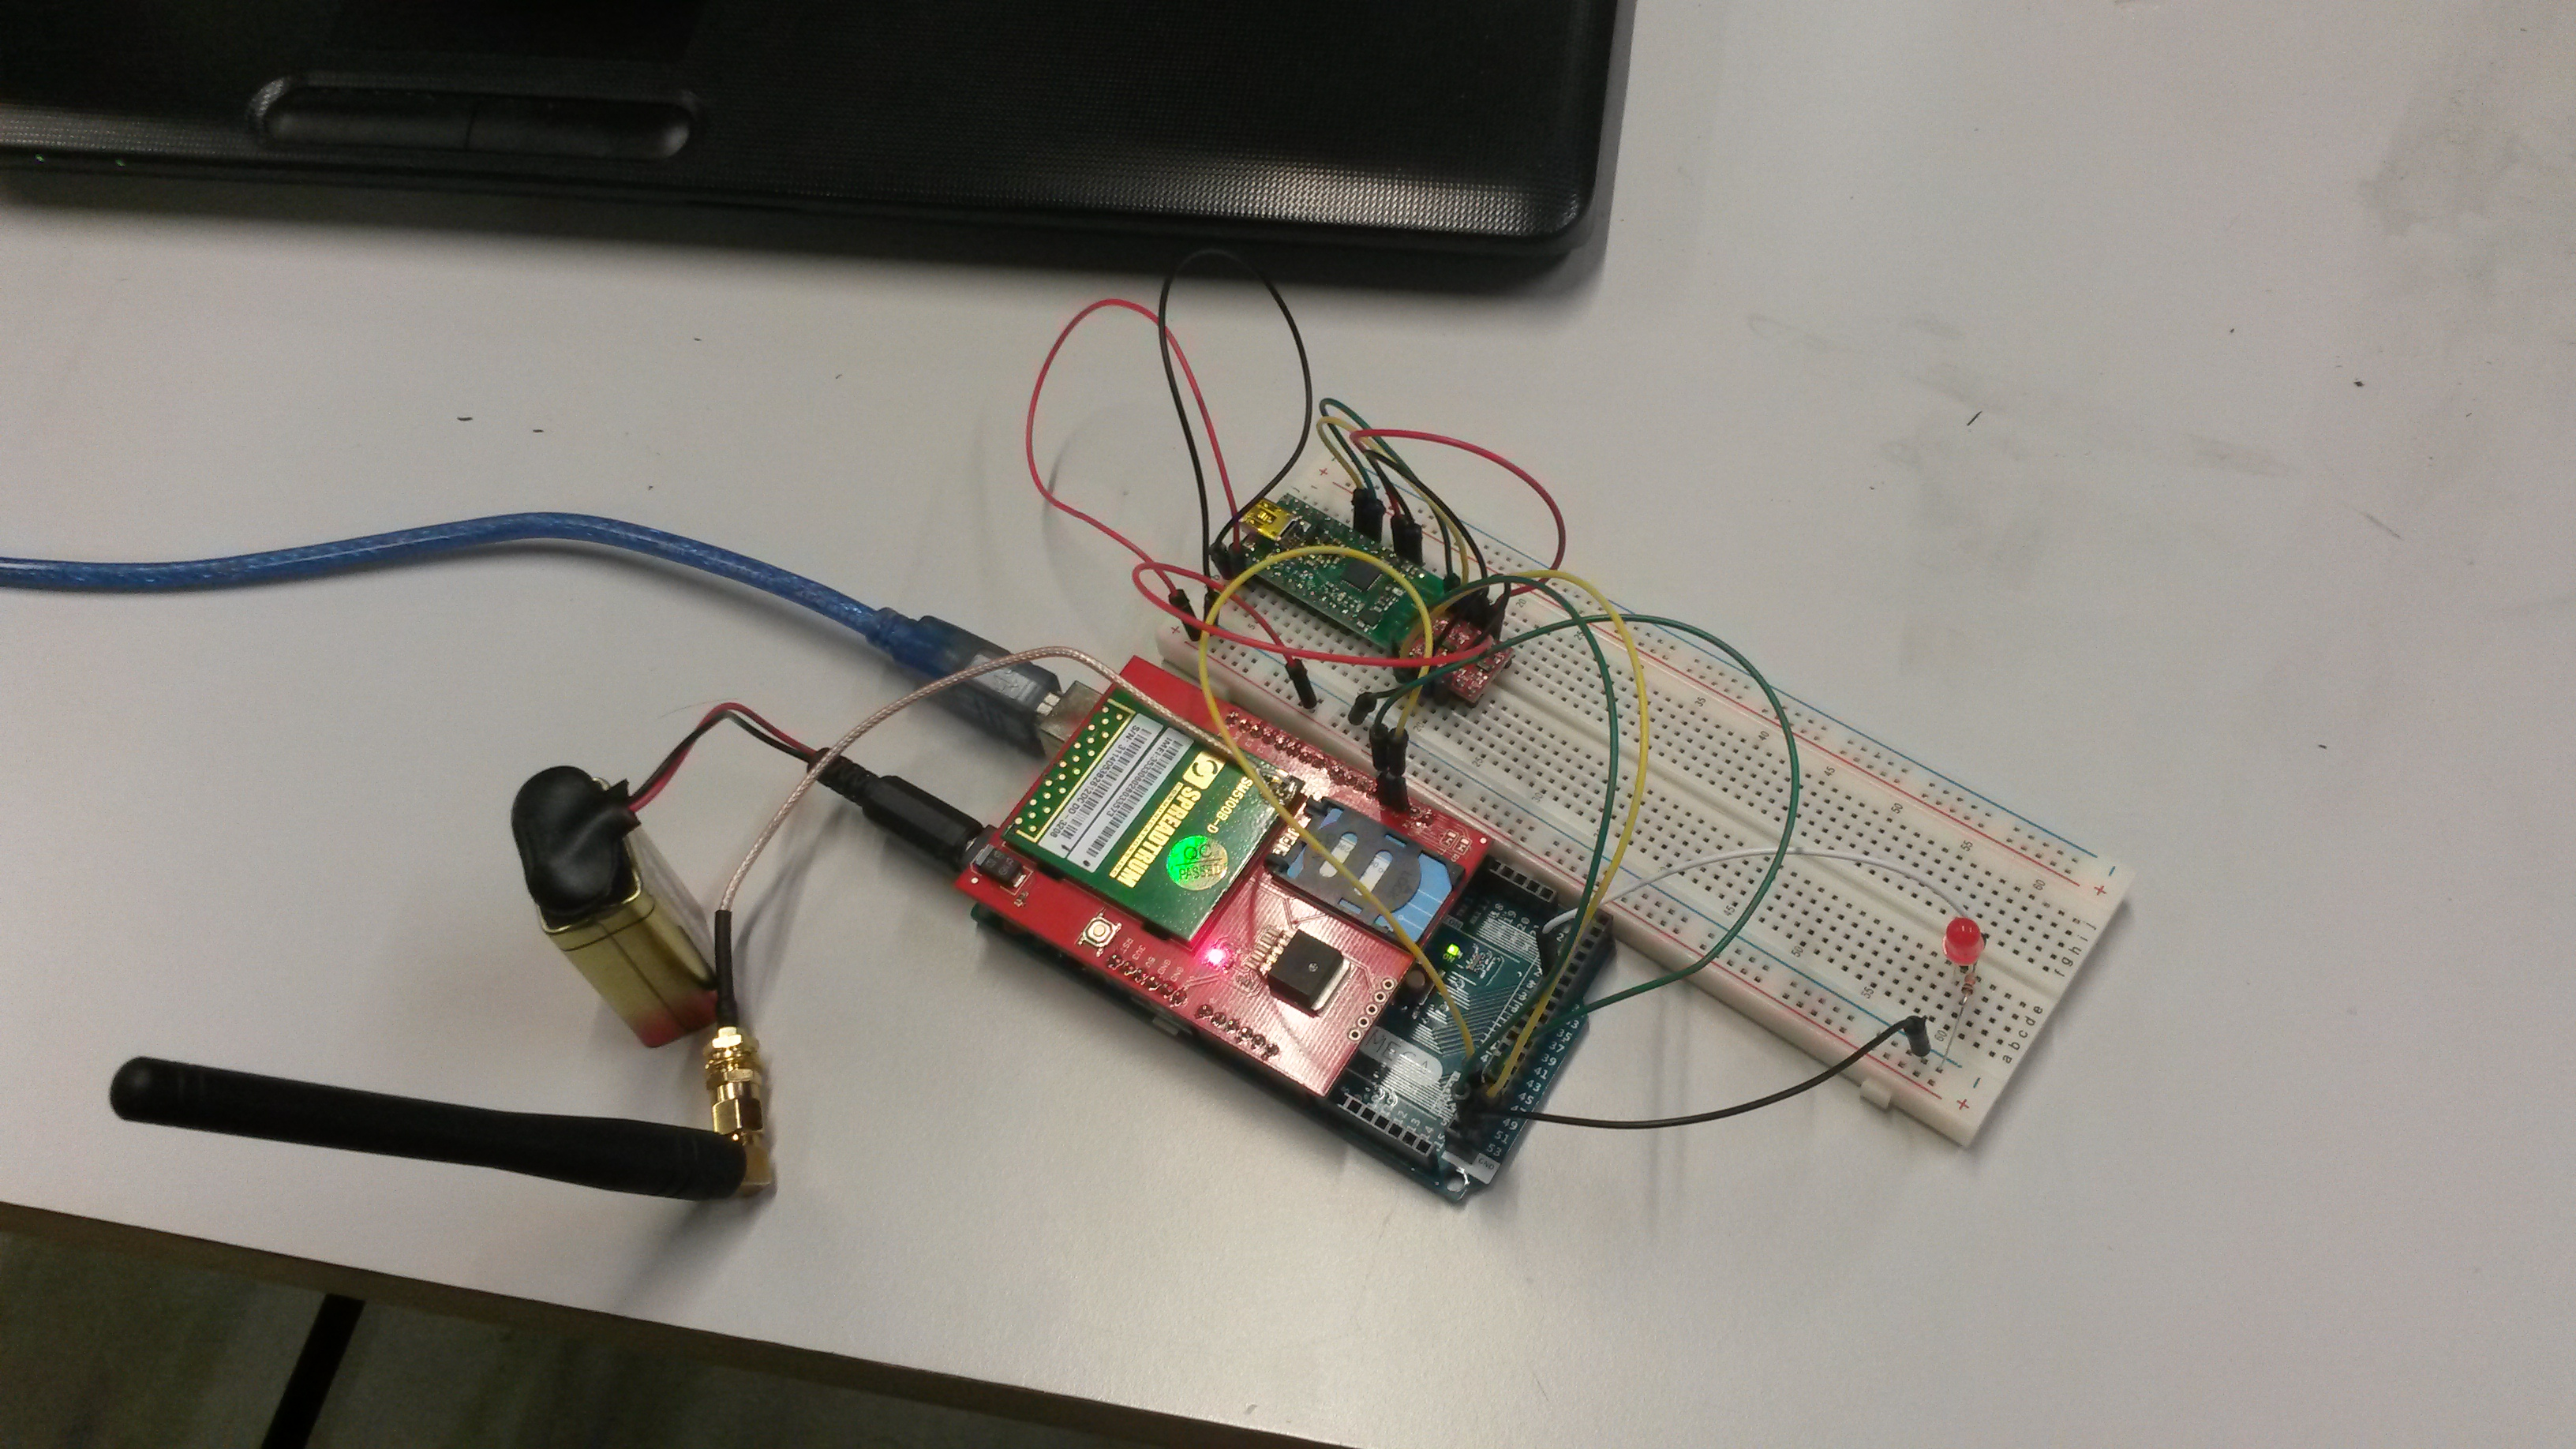
\includegraphics[height=5cm]{graphics/gsmArduino.jpg}
\end{frame}

\begin{frame}{Status}
\begin{columns}[T] % contents are top vertically aligned
     \begin{column}[T]{6cm} % each column can also be its own environment
		\begin{itemize}
		\item Web API, Jason format:
			\{\\
				"Data": "xxx"\\
				"Time": "2014:10:27:14:22"\\
			\}
		\item Development environment for Wixel
		\item Software architecture
		\item Layered structure designing
		\end{itemize}
	\end{column}
     \begin{column}[T]{4cm} % alternative top-align that's better for graphics
          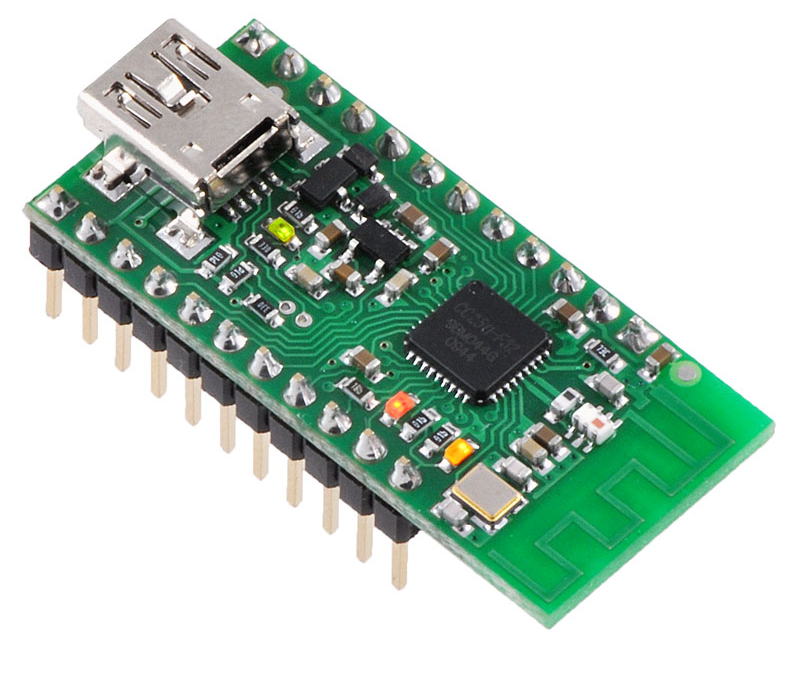
\includegraphics[height=3cm]{graphics/wixel.png}
          \cite{wixel}
     \end{column}
     \end{columns}
%What have you done?  What is the current state?  Is there any interesting/hard problems
%that need to be solved?  How are you going to solve them?
\end{frame}

\begin{frame}{Interesting problems}
\begin{itemize}
\item Making the design modular
\item Multiple communication methods.
	\begin{itemize}
	\item GSM
	\item Iridium
	\item Radio
	\end{itemize}
\item Minimizing power consumption
\end{itemize}
\end{frame}

\begin{frame}{Tasks remaining}
%What is left to be done?  This should be broken down by the time remaining in class.
	\begin{tabular}{ | l | l | l |}
    \hline
    \textbf{Task} & \textbf{Priority} & \textbf{Estimated time}\\ \hline
    Software implementation & 1 & 4 workdays \\ \hline
    Functions test & 1 - 2 & - \\ \hline
	Hardware construction & 1 - 3 & 1 workday\\ \hline
	Field test & 4 & 1 workday\\ \hline
    \end{tabular}
\end{frame}

\begin{frame}{References}
Thank you for your time.
Questions?
\bibliographystyle{IEEEtran}
{\tiny \bibliography{references}}
\end{frame}

\end{document}
